\documentclass{article}
\usepackage{graphicx} % Required for inserting images

\title{Homework 4}
\author{Ayman Tawaalai }
\date{February 2024}

\begin{document}

\maketitle

\section{Introduction}
The purpose of the given assignment is to study and implement Naive Bayes through practical means. The assignment states that the student must one hot encode and ngram the patient sequence data from homework 1. Once that is completed, it will serve as the input features of x. Next, K means clustering must be done and it will serve as the truth labels, y. Once the x and y values are attained, multinomial and gaussian naive bayes will be implemented separately.
\begin{figure}
    \centering
    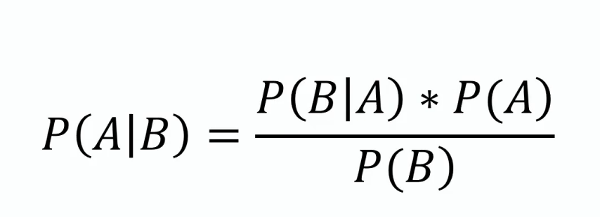
\includegraphics[width=0.5\linewidth]{1.png}
    \caption{Naive Bayes Formula}
    \label{fig:enter-label}
\end{figure}
\section{Naive Bayes}
Naive Bayes is a supervised machine learning classification model that uses probability. It works by taking in probabilities for predicted outcomes and uses those probabilities to determine if the given inputs are what is the expected output. An example of this can be seen through spam email classification. In this scenario, emails are scanned and each word in the email will weigh the probability of it being real or spam. Whichever has the higher probability will be sorted into the respective category. There are two types of Naive Bayes. The email example most similarly fits with multinomial naive bayes because of the use of discrete variables. Gaussian Naive Bayes focus on continuous variables. It works by getting the probability dense function for each class and then uses it for classification purposes.

\section{Implementation}
Since the working data is housed in the third column, we will load the files using pandas. Once all the strings are parsed to floats, dummies is used for one hot conversion. 
\begin{figure}
    \centering
    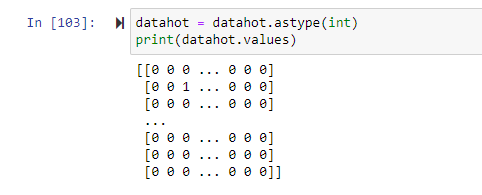
\includegraphics[width=0.5\linewidth]{2.png}
    \caption{One Hot Conversion}
    \label{fig:enter-label}
\end{figure}
The next step will be to conduct ngram as shown in figure three. 
\begin{figure}
    \centering
    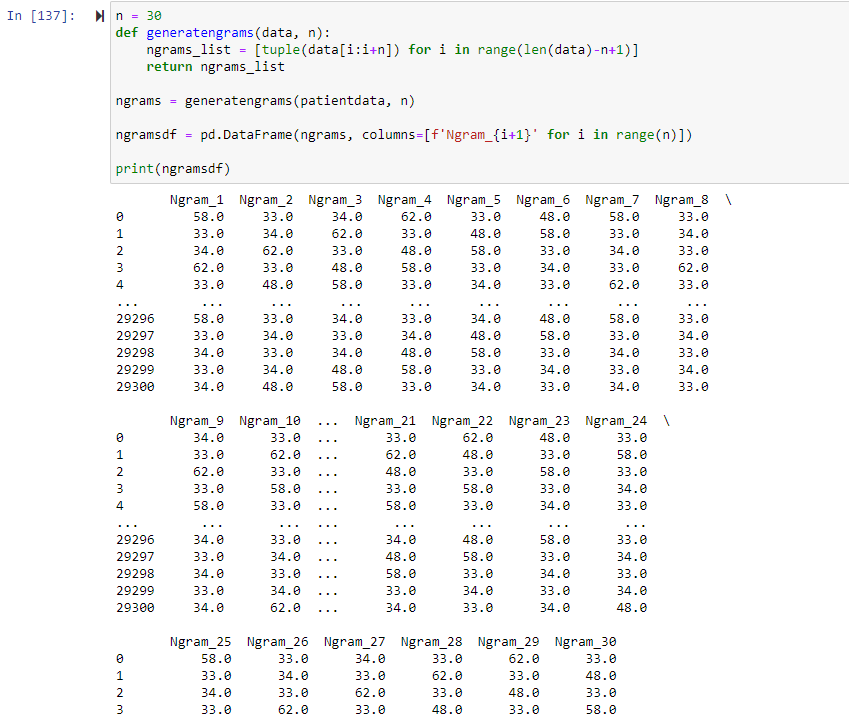
\includegraphics[width=0.5\linewidth]{3.png}
    \caption{NGram conversion of orginal patient data}
    \label{fig:enter-label}
\end{figure}
Since the x values have now been generated it is now time to get the y values. The one hot was sent into the k means function and the user would have to input how many clusters they would like and how many iterations the model should run for. After K means is completed the y values have been generated. With both x and y values, it is time to begin Naive Bayes. 
\begin{figure}
    \centering
    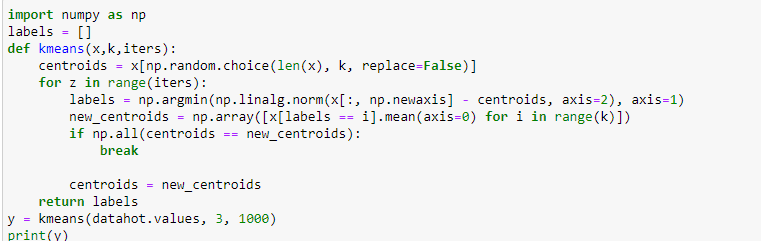
\includegraphics[width=0.5\linewidth]{4.png}
    \caption{KMeans implementation}
    \label{fig:enter-label}
\end{figure}

The first implementation will be for multinomial. The main work horse is the fit function. The function will take in both x and y values, split into training sets and testing sets, and uses Laplace smoothing to calculate the class probabilities. It places all the feature probabilities into an array and will return that array along with the class probability and classes itself. The predict function will take the final probabilities, along with the test data, and then predict the test labels for each test. Accuracy is then computed using SK learn.

\begin{figure}
    \centering
    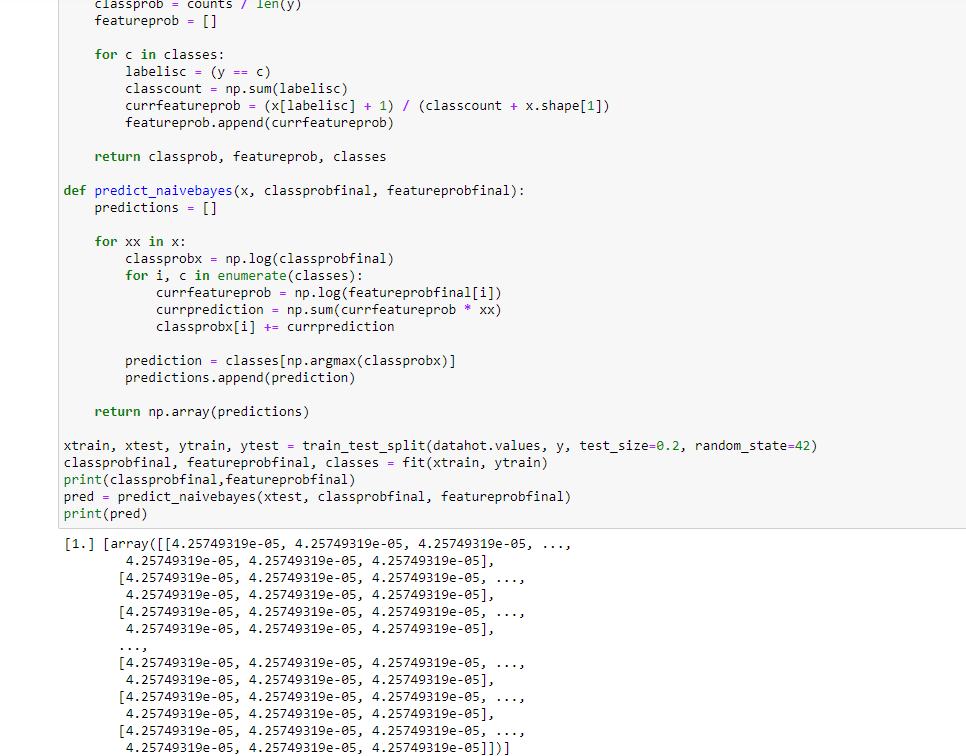
\includegraphics[width=0.5\linewidth]{5.png}
    \caption{Multinomial Naive Bayes implementation}
    \label{fig:enter-label}
\end{figure}

The second implementation will be for gaussian. The same x and y values would be used, but a new fit function would have to be made. The gaussianfit function will return the feature means and standard deviation but is different from the fit function where it will return the feature probabilities. The predict function will take in the finals returned by the fit function and use the pdf function for calculation. The pdf function includes an epsilon to avoid divide by zero errors which were an issue. It will use that calculation to predict the class labels and append that to the predictions array, which is what is returned.
\begin{figure}
    \centering
    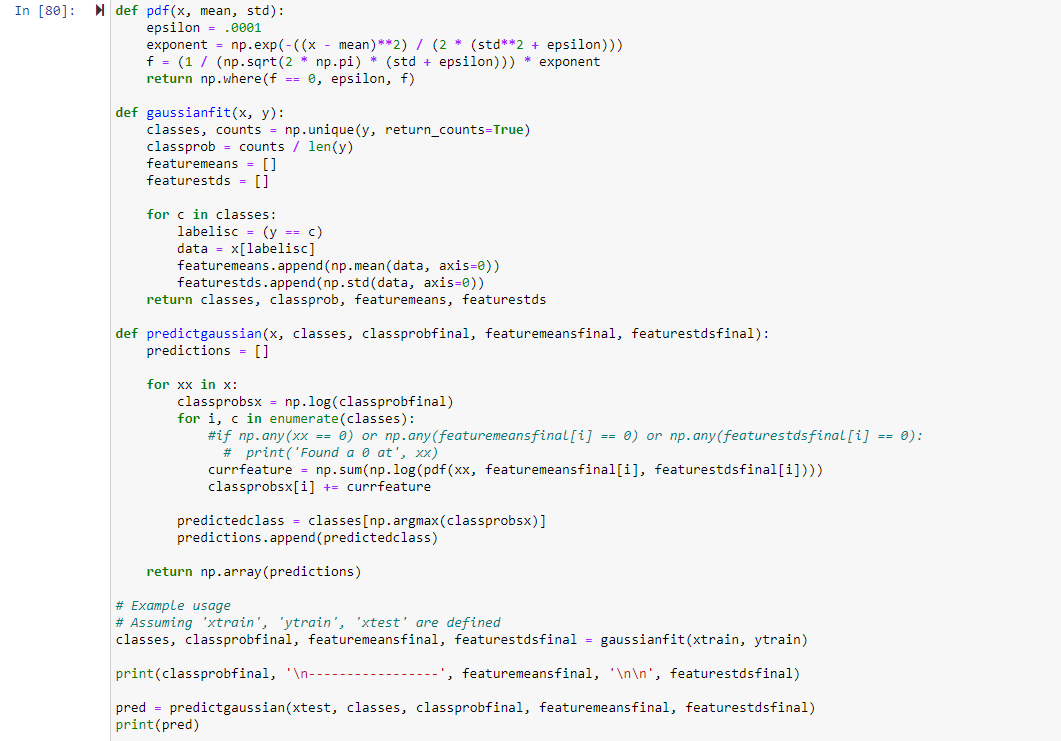
\includegraphics[width=0.5\linewidth]{6.png}
    \caption{Gaussia Naive Bayes implementation}
    \label{fig:enter-label}
\end{figure}

\section{WEKA}
To load the data into weka, some changes were made to the pd loading code. The new changes will now have the third column, along with the key value of the classes, be written into a csv file. That csv file will be loaded for naive bayes in weka. The results show that only 13\% of instances were classified correctly. Furthermore, the summary provided by weka suggests that Naive Bayes does not work best for the data set.
\begin{figure}
    \centering
    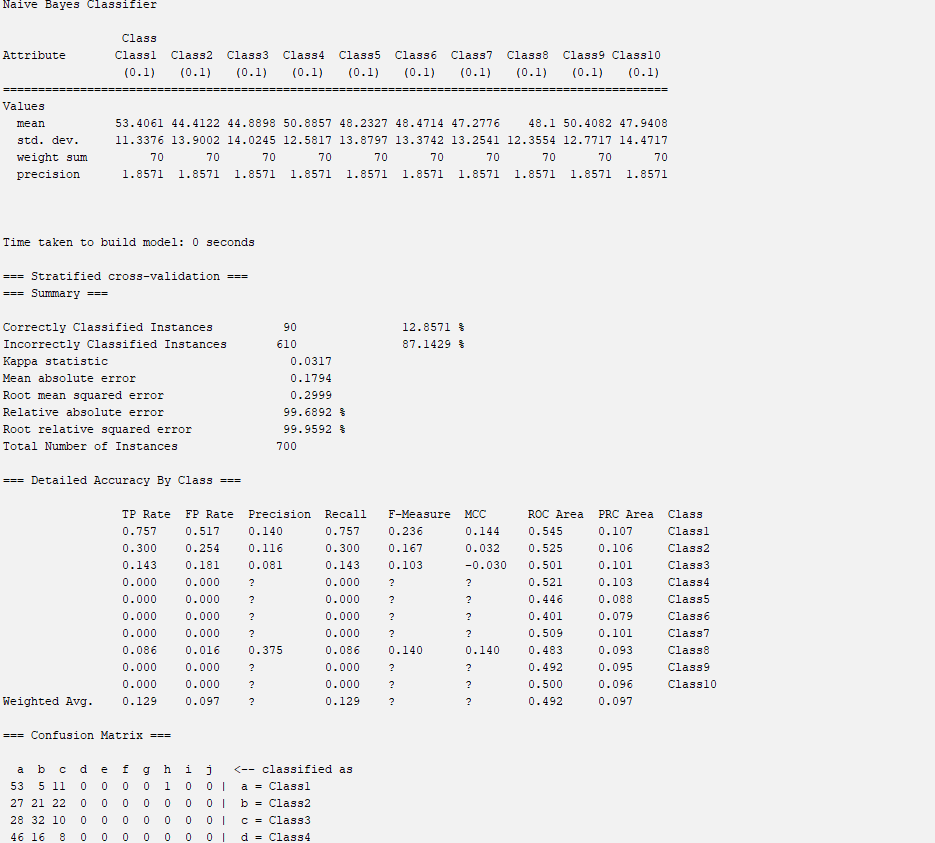
\includegraphics[width=0.5\linewidth]{7.png}
    \caption{Weka Summary}
    \label{fig:enter-label}
\end{figure}
\section{Conclusion}
The purpose of this assignment was to implement both version of Naive Bayes in python to better understand how the model works from a white box perspective. The python implementation had both multinomial and Gaussian to accomplish this. The low accuracy was further reflected in Weka where it showed a low accuracy there as well in the summary. In conclusion, the given data set does not bode well with Naive Bayes tries to accomplish.
\end{document}
